\chapter{Applications}

\fbox{
    \parbox{\textwidth}
    {
        Chapter Overview
        \begin{itemize}
            \item Empirical analysis of BayesCNN with normal architecture for Image Super Resolution.
            \item Empirical analysis of BayesCNN with normal architecture for Generative Adversarial Networks.
        \end{itemize}
    }
}

\pagebreak



\section{BayesCNN for Image Super Resolution}

The task referred to as Super Resolution (SR) is the recovery of a High-Resolution (HR) image from a given Low-Resolution (LR) image. It is applicable to many areas like medical imaging \citet{10.1007/978-3-642-40760-4_2}, face recognition \citet{1203152} and so on.

There are many ways to do a single image super-resolution and detailed benchmarks of the methods are provided by Yang \citet{Yang2014SingleImageSA}. Following are the major ways to do a single image super-resolution:\\ 

\textbf{Prediction Models}: These models generate High-Resolution images
from Low-Resolution inputs through a predefined mathematical formula. No training data is needed for such models. Interpolation-based methods (bilinear, bicubic, and Lanczos) generate HR pixel intensities by weighted averaging neighbouring LR pixel values are good examples of this method.\\

\textbf{Edge Based Methods}: Edges are one of the most important features for any computer vision task. The High-Resolution images learned from the edge features high-quality edges and good sharpness. However, these models lack good colour and texture information.\\

\textbf{Patch Based Methods}: Cropped patches from Low-Resolution images and High-Resolution images are taken from training dataset to learn some mapping function. The overlapped patches are averaged or some other techniques like Conditional Random Fields \cite{lafferty2001conditional} can be used for better mapping of the patches.  


\subsection{Our Approach}

We build our work upon \citet{DBLP:journals/corr/ShiCHTABRW16} work that shows that performing Super Resolution work in High-Resolution space is not the optimal solution and it adds the computation complexity. We used a Bayesian Convolutional Neural Network to extract features in the Low-Resolution space. We use an efficient sub-pixel convolution layer, as proposed by \citet{DBLP:journals/corr/ShiCHTABRW16}, which learns an array of upscaling filters to upscale the final Low-Resolution feature maps into the High-Resolution output. This replaces the handcrafted bicubic filter in the Super Resolution pipeline with more complex upscaling filters specifically trained for each feature map, and also reduces the computational complexity of the overall Super Resolution operation.

The hyperparameters used in the experiments are mentioned in the Appendix A section in details.

\begin{figure*}[htbp]
\begin{center}
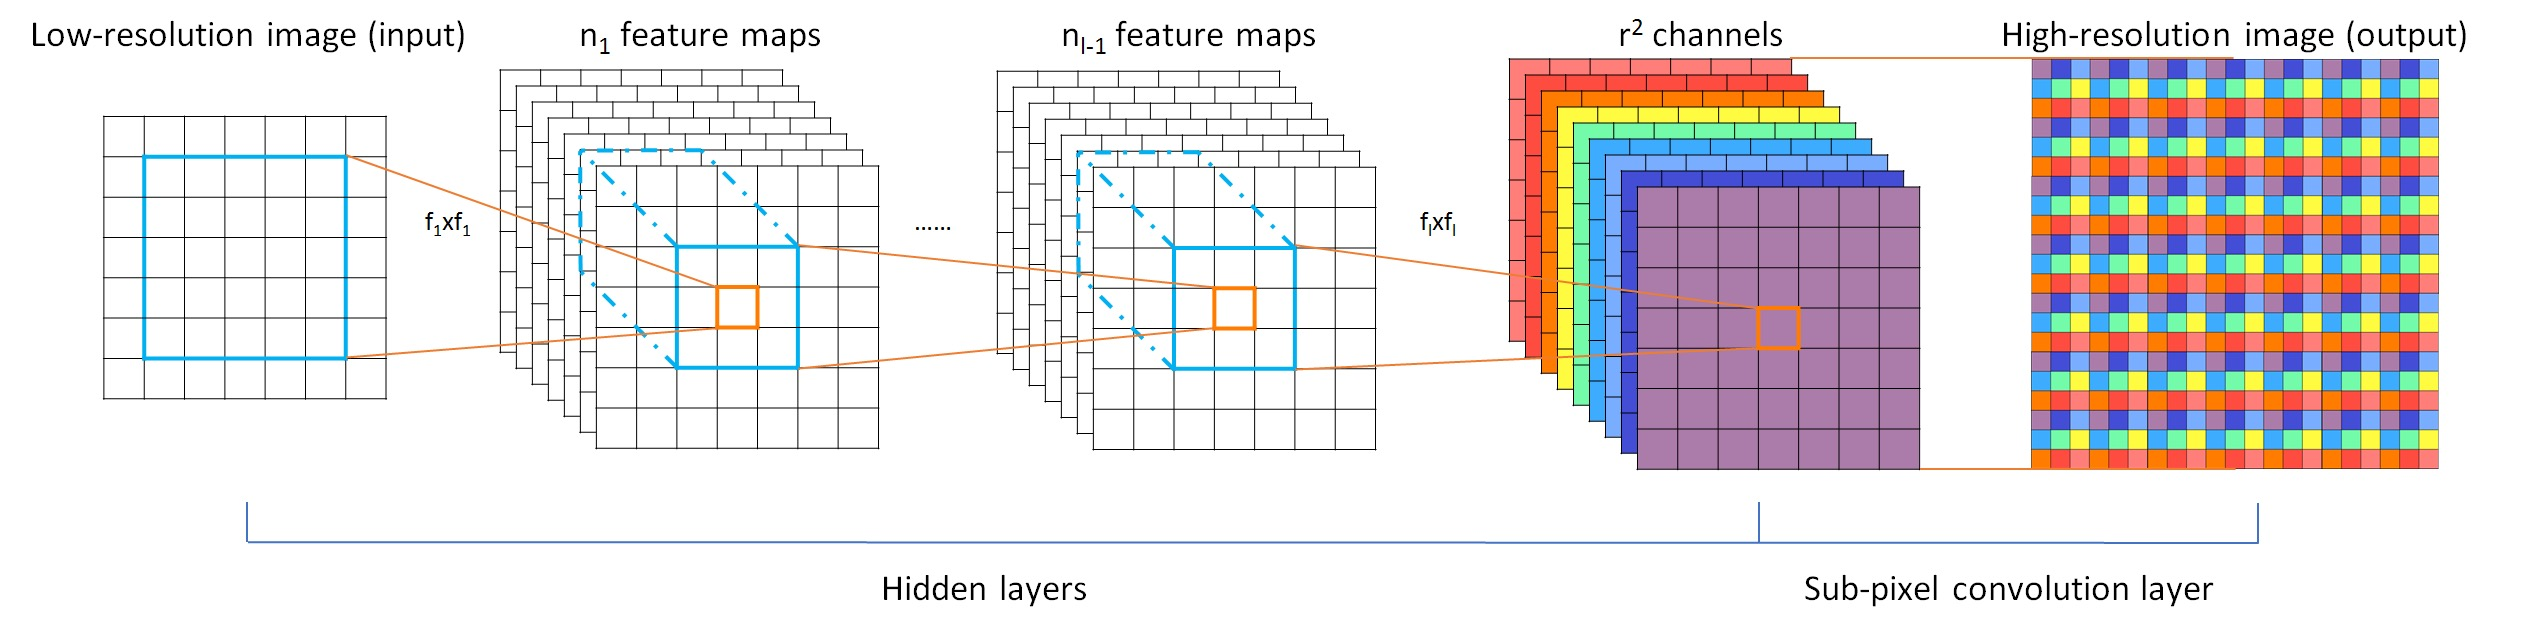
\includegraphics[width=1.0\linewidth]{Chapter6/Figs/networkstructure.jpg}
\caption{The proposed efficient sub-pixel convolutional neural network (ESPCN) \cite{DBLP:journals/corr/ShiCHTABRW16}, with two convolution layers for feature maps extraction, and a sub-pixel convolution layer that aggregates the feature maps from Low Resolution space and builds the Super Resolution image in a single step.}
\label{fig:networkstructure}
\end{center}
\end{figure*}

We used a four-layer convolutional model as mentioned in the paper \cite{DBLP:journals/corr/ShiCHTABRW16}. We replaced the convolution layer by Bayesian convolution layer and changed the forward pass that now computes the mean, variance and KL divergence. The PixelShuffle layer is kept same as provided by PyTorch and no changes have been made there.  

\begin{table}[H]
    \centering
    \renewcommand{\arraystretch}{2}
    \begin{tabular}{c c c c } 
 \hline
 layer type & width & stride & padding  \\ [0.5ex] 
 \hline
 convolution ($5\times5$) & 64 & 1 & 2 \\
 
 convolution ($3\times3$) & 64 & 1 & 1 \\
 
 
 convolution ($3\times3$) & 32 & 1 & 1 \\
 
 convolution ($3\times3$) & upscale factor * * 2 & 1 & 1  \\ [1ex] 
 \hline
\end{tabular}
\renewcommand{\arraystretch}{1.5}
\label{tab:SuperResolutionArchitecture}
\caption{Network Architecture for Bayesian Super Resolution}
\end{table}

Where \textit{upscale factor} is defined as a parameter. For our experiments, we take upscale factor = 3. 

\subsection{Empirical Analysis}

The Network architecture was trained on BSD300 dataset \cite{MartinFTM01} provided by the Berkeley Computer Vision Department. The dataset is very popular for Image Super-Resolution task and thus the dataset is used to compare the results with other work in the domain. 

\begin{figure}[H]
\begin{center}
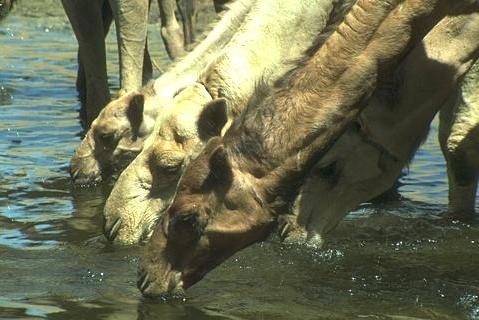
\includegraphics[height=.28\textheight]{Chapter6/Figs/camel_LR.png}
\label{fig:CamelLR}
\caption{Sample image in Low Resolution image space taken randomly from BSD 300 \cite{MartinFTM01} dataset.}
\end{center}
\end{figure}

\begin{figure}[H]
\begin{center}
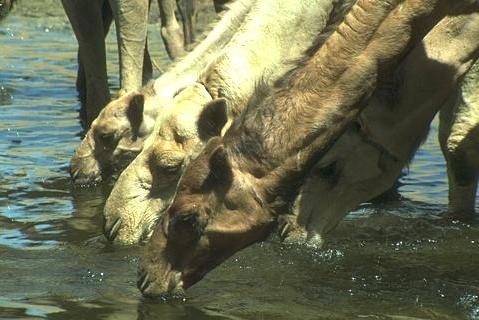
\includegraphics{Chapter6/Figs/camel_LR.png}
\label{fig:CamelSR}
\caption{Generated Super Resolution Image}
\end{center}
\end{figure}

The generated results with Bayesian Network is compared with the original paper and the results are comparable in terms of the number and the quality of the image generated. This application was to prove the concept that the Bayesian Networks can be used for the task of Image Super Resolution. Furthermore, the results are pretty good. 

Some more research is needed in the future to achieve state-of-the-art results in this domain which is out of the scope of this thesis work.


\section{BayesCNN for Generative Adversarial Networks}

Generative Adversarial Networks (GANs) \cite{goodfellow2014generative} can be used for two major tasks: to learn good feature representations by using the generator and discriminator networks as feature extractors and to generate natural images. The learned feature representation or generated images can reduce the number of images substantially for a computer vision supervised task. However, GANs were quite unstable to train in the past and that is why we base our work on the stable GAN architecture namely Deep Convolutional GANs (DCGAN) \cite{DBLP:journals/corr/RadfordMC15}. We use the trained Bayesian discriminators for image classification tasks, showing competitive performance with the normal DCGAN architecture.

\subsection{Our approach}

We based our work on the paper:  Unsupervised Representation Learning with Deep Convolutional Generative Adversarial Networks by  \citet{DBLP:journals/corr/RadfordMC15}. We used the architecture of a deep convolutional generative adversarial networks (DCGANs) that learns a hierarchy of representations from object parts to scenes in both the generator and discriminator.
The generator used in the Network is shown in Table \ref{tab:GeneratorArchitecture}. The architecture is kept similar to the architecture used in DCGAN paper \cite{DBLP:journals/corr/RadfordMC15}. Table \ref{tab:DiscriminatorArchitecture} shows the discriminator network with Bayesian Convolutional Layers. 

\begin{table}[H]
    \centering
    \renewcommand{\arraystretch}{2}
    \begin{tabular}{c c c c c} 
 \hline
 layer type & width & stride & padding & nonlinearity \\ [0.5ex] 
 \hline
 ConvolutionTranspose ($4\times4$) & ngf * 8 & 1 & 0  & ReLU \\ 
 

 ConvolutionTranspose ($4\times4$) & ngf * 4 & 2 & 1  & ReLU \\
 
 
 ConvolutionTranspose ($4\times4$) & ngf * 2 & 2 & 1 & ReLU \\
 
 ConvolutionTranspose ($4\times4$) & ngf & 2 & 1  & ReLU \\
 
 ConvolutionTranspose ($4\times4$) & nc & 2 & 1 & TanH \\ [1ex] 
 \hline
\end{tabular}
\renewcommand{\arraystretch}{1}
\caption{Generator architecture as defined in the paper. \cite{DBLP:journals/corr/RadfordMC15}}
\label{tab:GeneratorArchitecture}
\end{table}

where \textit{ngf} is the number of generator filters which is chosen to be 64 in our work and \textit{nc} is the number of output channels which is set to 3. 

\begin{table}[H]
    \centering
    \renewcommand{\arraystretch}{2}
    \begin{tabular}{c c c c c} 
 \hline
 layer type & width & stride & padding & nonlinearity \\ [0.5ex] 
 \hline
 Convolution ($4\times4$) & ndf & 2 & 1  & LeakyReLU \\ 
 

 Convolution($4\times4$) & ndf * 2 & 2 & 1  & LeakyReLU \\
 
 
 Convolution ($4\times4$) & ndf * 4 & 2 & 1 & LeakyReLU \\
 
 Convolution ($4\times4$) & ndf * 8 & 2 & 1  & leakyReLU \\
 
 ConvolutionTranspose ($4\times4$) & 1 & 1 & 0 & Sigmoid \\ [1ex] 
 \hline
\end{tabular}
\renewcommand{\arraystretch}{1}
\caption{Discriminator architecture with Bayesian Convolutional layers}
\label{tab:DiscriminatorArchitecture}
\end{table}

where \textit{ndf} is the number of discriminator filters and is set to 64 as default for all our experiments. 

\subsection{Empirical Analysis}

The images were taken directly and no pre-processing was applied to any of the images. Normalization was applied with value 0.5 to make the data mean centred. A batch size of 64 was used along with Adam \citep{kingma2014adam} as an optimizer to speed up the training. All weights were initialized from a zero-centred Normal distribution with standard deviation equal to 1. We also used LeakyReLU as mentioned in the original DCGAN paper \cite{DBLP:journals/corr/RadfordMC15}. The slope of the leak in LeakyReLU was set to 0.2 in all models. We used the learning rate of 0.0001, whereas in paper 0.0002 was used instead. Additionally, we found leaving the momentum term $\beta_1$ at the suggested value of 0.9 resulted in training oscillation and instability while reducing it to 0.5 helped stabilize training (also taken from original paper \cite{DBLP:journals/corr/RadfordMC15}).

The hyperparameters used in the experiments is mentioned in the Appendix A section in details.
The fake results of the generator after 100 epochs of training is shown in Figure 6.4. To compare the results, real samples are shown in Figure 6.5. The loss in case of a Bayesian network is higher as compared to the DCGAN architecture originally described by the authors. However, upon looking at the results, there are no comparison that can be drawn from the results of the two networks. Since GANs are difficult to anticipate just by the loss number, the comparison cannot be made. The results are pretty comparable for the Bayesian models and the original DCGAN architecture. 

\begin{figure}[H]
\begin{center}
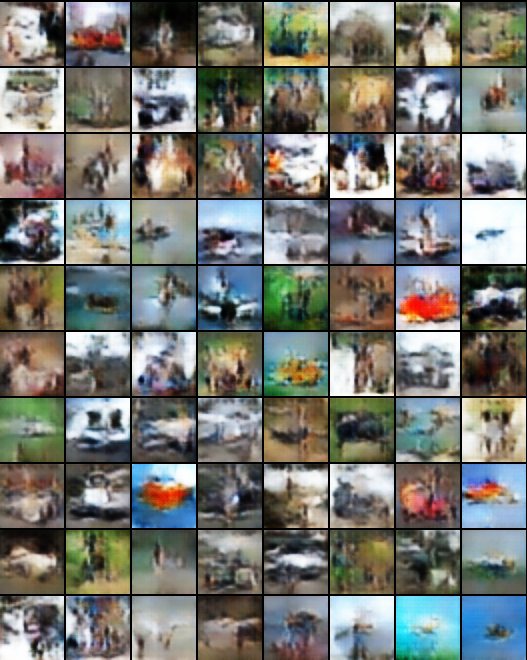
\includegraphics[height=.88\textheight]{Chapter6/Figs/fake_samples.png}
\label{fig:FakeSamples}
\caption{Fake Samples generated from the Bayesian DCGAN model trained on CIFAR10 dataset}
\end{center}
\end{figure}

\begin{figure}[H]
\begin{center}
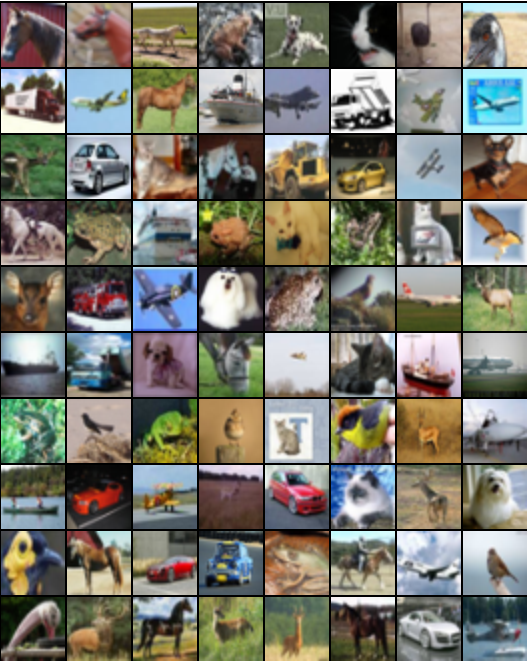
\includegraphics[height=.88\textheight]{Chapter6/Figs/realsamples.png}
\label{fig:RealSamples}
\caption{Real Samples taken from CIFAR10 dataset}
\end{center}
\end{figure}



